Las direcciones \texttt{IPs} son los numeros que nuestras computadoras, servidores, telefonos, impresoras y sensores permiten que se comuniquen entre si. Sin direcciones \texttt{IP}, tendriamos que copiar los datos a un dispositivo de manera manual. No podrian enviarse datos sin intervención humana.
\section*{IPs Privadas y Publicas} 
\subsection*{IPs Privadas}
Una dirección IP privada es una dirección IP reservada para uso interno detras de un enrutador u otro dispositivo de traducción de direcciones de red (NAT)\footnote{\texttt{NAT}=\textbf{N}etwork \textbf{A}ddress \textbf{T}ranslation}, aparte del público. A veces también se les conoce como dirección \textbf{IP Local}. La IANA (Internet Assigned Numbers Authority) reserva los siguientes bloques para su uso privado:
\begin{itemize}
\item \texttt{10.0.0.0} a \texttt{10.255.255.255}
\item \texttt{172.16.0.0} a \texttt{172.31.255.255}
\item \texttt{192.168.0.0} a \texttt{192.168.255.255}
\end{itemize}
El primer conjunto de direcciones IP permite mas de 16 millones de direcciones, el segundo mas o menos 1 millón y mas de 65000 para el último. Estas direcciones pueden repetirse en redes distintas, en cuyo caso no habrá conflictos debido a que las redes se encuentran separadas.
\subsection*{IPs Publicas}
Una IP pública es una dirección que el router recibe de su ISP (Internet Service Provider). Se requieren direcciones de IP publicas para cualquier hardware de red de acceso publico, como los enrutadores domesticos y los servidores que alojan sitios web. Estas son siempre unicas, es decir no se pueden repetir. Dos equipos con IP de este tipo pueden conectarse directamente entre sí.

\subsubsection*{Funcionamiento}
Podemos decir que una IP privada (a grosso modo) es lo ``mismo'' que una IP publica. Básicamente un identificador único para todos los dispositivos detras de un enrutador u otro dispositivo que sirve direcciones IP. Como las redes distintas pueden tener IPs iguales (privadas), ya que no son enrutables el primero evitará que los dispositivos con IP privadas se comuniquen con otra mas allá del enrutador. Como la IP privada no puede acceder a Internet, necesita una dirección que pueda llegar al resto del mundo aqui entra la IP publica.  Esto permite que los dispositivos en una red doméstica transmitan información de ida y vuelta entre al enrutador y el ISP.

\section*{IPs Dinámicas y Estáticas}
\subsection*{IPs Dinámicas} 
Es aquella que cambia cada cierto tiempo (usadas en empresas o servidores que reciben mucho flujo). Así la IP cambia en función a las necesidades del servidor, siendo util en el balanceo de carga. Las PCs tienen diferentes IPs para poder conectarse a un servidor, la mayoría dependen de esto. Aunque es probable que el ISP cambie estas direcciones IP, e menudo permanecen iguales durante semanas, meses o incluso años y a veces el usuario no se da cuenta.
\subsection*{IPs Estáticas}
Es asignada por el usuario manualmente o por el servidor de red (ISP) con base a la dirección MAC del cliente.

\begin{figure}[H]
  \centering
  \begin{minipage}[b]{0.4\textwidth}
    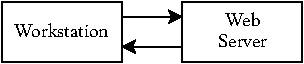
\includegraphics[page=1,scale=0.7]{ESTATICO.pdf}
    \caption{IP Estática}
  \end{minipage}
  \begin{minipage}[b]{0.4\textwidth}
    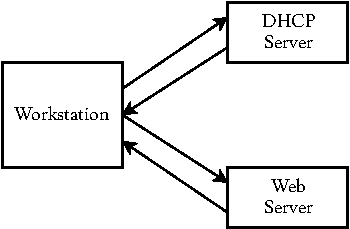
\includegraphics[page=1,scale=0.7]{DINAMICO.pdf}
    \caption{IP Dinámica}
  \end{minipage}
\end{figure}

\section*{IPv6}
Su función es exactamente la misma que su predecesor \texttt{IPv4}. Se compone de la siguiente manera:


\begin{center}
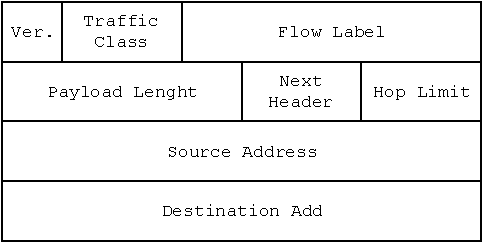
\includegraphics[page=1,scale=0.8]{IPv6.pdf}
\end{center}

\begin{itemize}
\item \texttt{Version}(4Bits): Indica la versión del protocolo \texttt{IPv6}. Tiene el mismo tamaño que en \texttt{IPv4}.
\item \texttt{Traffic Class}(8Bits): Puede tomar valores diferentes para permitir que el nodo de origen diferencie entre los paquetes generados por él al asociarles diferentes prioridades de entrega. Es usado por el nodo origen y enrutadores.
\item \texttt{Flow Label}(20Bits): Se usa para etiquetar un conjunto de paquetes que pertenecen al mismo flujo. Un flujo se identifica de forma exclusiva por la dirección de origen y una etiqueta de flujo.
\item \texttt{Payload Length}(16Bits): Contiene la longitud del campo de datos en octetos que sigue al encabezado.
\item \texttt{Next Header}(8Bits): Identifica el encabezado inmediatamente despues del encabezado \texttt{IPv6} y ubicado al comienzo
\item \texttt{Hop Limit}(8Bits): Cumple la misma función que el \texttt{TTL}.
\item \texttt{Source Address}(128Bits): La dirección de origen es la dirección IPv6 de 128 bits de la fuente original del paquete.
\item \texttt{Destination Address}(128Bits): El campo Dirección de destino indica la dirección IPv6 del destino final (en la mayoría de los casos). Todos los nodos intermedios pueden usar esta información para enrutar correctamente el paquete.
\end{itemize}

%\begin{figure}[H]
%\centering
%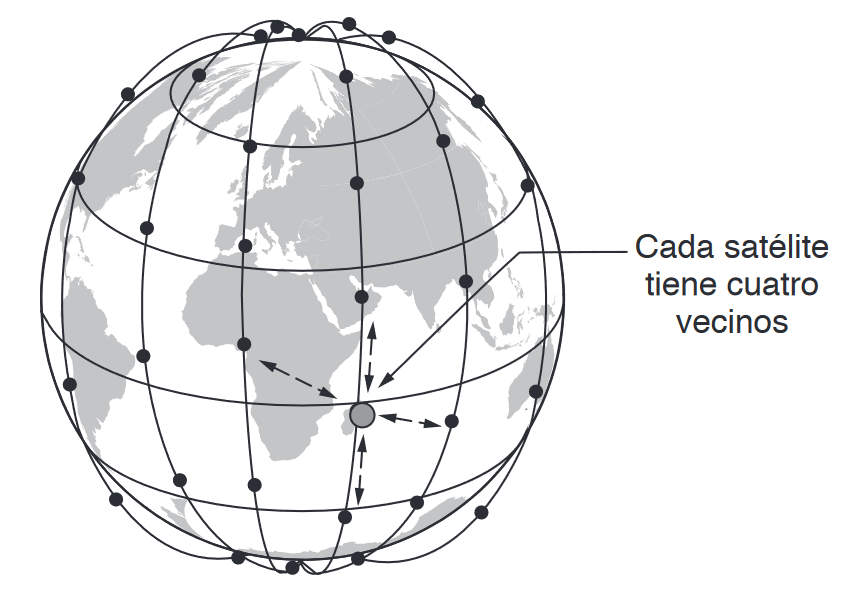
\includegraphics[page=1,scale=0.7]{SATELITES2.png}
%\caption{Satélites Iridium \textit{(Redes de Computadoras, Tanenbaum 4ta Edición, Pagina 105)}}
%\end{figure}

%\begin{figure}[H]
%\centering
%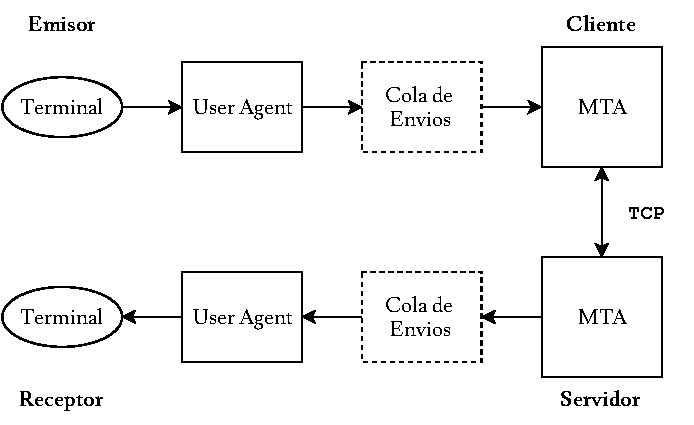
\includegraphics[page=1,scale=0.7]{SMTP.pdf}
%\caption{Esquema de funcionamiento de SMTP}
%\end{figure}
